% Show important proofs
% show the foundational sätze they use

\begin{frame}{Reminder: Definition of Orthogonal Projection} % How do we define it?
  \begin{align*}
    \Pi_{\mathcal{G}}y = \arg\min_{g \in \mathcal{G}} \|y - g\|^2
= \arg\min_{g \in \mathcal{G}} \mathbb{E}[(y(\boldsymbol{X}) - g(\boldsymbol{X}))^2].
\end{align*}
  \begin{itemize}
    \item $\mathcal{G}$ : linear subspace of $\mathcal{L}^2$ we project onto
    \item $g$ all functions in the subspace
  \end{itemize}
\end{frame}



\begin{frame}{Equality to Hoeffding Decomposition} % How does it relate to Hoeffding?
  \begin{block}{Hoeffding Decomposition}
    \begin{align}
    y(\boldsymbol{X})
=
\sum_{A \subseteq D} 
y_A(\boldsymbol{X}_A),
\qquad
D := \{1,\dots,N\},
\end{align}
where, for each $A \subseteq D$, the component function $y_A$ is defined by:
\begin{align}\label{eq:hoeffding_components}
    y_A(\boldsymbol{X}_A)
=
\sum_{B \subseteq A}
(-1)^{|A|-|B|}
\,\mathbb{E}\!\left[
  y(\boldsymbol{X}) 
  \,\middle|\, 
  \boldsymbol{X}_B
\right],
\end{align}
  where $y_u$ are orthogonal components.
  \end{block}
  \begin{itemize}
    \item Classical fANOVA and Hoeffding decomposition yield same components under zero-centered inputs
    \item Both assume independence of input variables
  \end{itemize}
  
\end{frame}

\begin{frame}{Hoeffding Decomposition Example} % Example of Hoeffding decomposition
  \begin{align*}
    y(x_1, x_2) = 2x_1 + x_2^{2} + x_1 x_2
  \end{align*}
  \begin{align*}
    % --- constant component
    y_{\emptyset}
    &= \mathbb{E}[y(X_1,X_2)] 
     = 2\,\mathbb{E}[X_1] + \mathbb{E}[X_2^2] + \mathbb{E}[X_1 X_2] 
     = 1,
    \\[1.2em]
    % --- first-order component for X1
    y_{\{1\}}(x_1)
    &= \sum_{B \subseteq \{1\}} (-1)^{1-|B|}
       \,\mathbb{E}[y(\boldsymbol{X})\,|\,X_B] = -\,\mathbb{E}[y] + \mathbb{E}[y|X_1=x_1] \\[2pt]
    &= -1 + (2x_1 + \mathbb{E}[X_2^2] + x_1\mathbb{E}[X_2]) = 2x_1,
    \\[1.2em]
    % --- first-order component for X2
    y_{\{2\}}(x_2)
    &= \sum_{B \subseteq \{2\}} (-1)^{1-|B|}
       \,\mathbb{E}[y(\boldsymbol{X})\,|\,X_B] -\,\mathbb{E}[y] + \mathbb{E}[y|X_2=x_2] \\[2pt]
    &= -1 + (2\mathbb{E}[X_1] + x_2^2 + x_2\mathbb{E}[X_1]) = x_2^2 - 1.
\end{align*}
\end{frame}

\begin{frame}
  \begin{align*}
    % --- second-order interaction component
    y_{\{1,2\}}(x_1,x_2)
    &= \sum_{B \subseteq \{1,2\}} (-1)^{2-|B|}
       \,\mathbb{E}[y(\boldsymbol{X})\,|\,X_B] \\[2pt]
    &= (+1)\,\mathbb{E}[y] 
     - \mathbb{E}[y|X_1=x_1]
     - \mathbb{E}[y|X_2=x_2]
     + y(x_1,x_2) \\[2pt]
    &= 1 - (2x_1+1) - (x_2^2) + (2x_1+x_2^2+x_1x_2) \\[2pt]
    &= x_1 x_2.
\end{align*}

\[
y(x_1,x_2)
= y_{\emptyset} + y_{\{1\}}(x_1) + y_{\{2\}}(x_2) + y_{\{1,2\}}(x_1,x_2)
= 1 + 2x_1 + (x_2^2 - 1) + x_1 x_2
\]

\end{frame}



\begin{frame}
  Substituting the basis functions:
  \begin{align*}
   y(x_1,x_2)  = \underbrace{c_0}_{y_0}
   &+ \underbrace{\big(c_{1,1}\,x_1 
                     + c_{1,2}\,(x_1^2 - 1)\big)}_{y_1(x_1)} \\[0.5em]
   &\quad
   + \underbrace{\big(c_{2,1}\,x_2 
                     + c_{2,2}\,(x_2^2 - 1)\big)}_{y_2(x_2)} \\[0.5em]
   &\quad
   + \underbrace{c_{12,11}\,\left(\frac{\rho (x_1^2 + x_2^2)}{1 + \rho^2} 
                         - x_1 x_2 
                         + \frac{\rho(\rho^2 - 1)}{1 + \rho^2}\right)}_{y_{12}(x_1,x_2)}.
\end{align*}
Find weights to recover original polynomial while fulfilling zero-mean and hierarchical orthogonality:
\[
y(x_1,x_2) = a_0 + a_1 x_1 + a_2 x_2 
   + a_{11} x_1^2 + a_{22} x_2^2 + a_{12} x_1 x_2 
\]

\end{frame}

\begin{frame}{Coefficient Matching}
  The corresponding weights can be found via coefficient matching. Start from the interaction term:
      \begin{align*}
-\,c_{12, 11} &= a_{12} &\Rightarrow\quad c_{12, 11} &= -a_{12} \\[0.5em]
c_{1,2} + c_{12, 11}\,\tfrac{\rho}{1+\rho^2} &= a_{11} 
&\Rightarrow\quad c_{1,2} &= a_{11} + \tfrac{\rho}{1+\rho^2}a_{12} \\[0.5em]
c_{2,2} + c_{12, 11}\,\tfrac{\rho}{1+\rho^2} &= a_{22} 
&\Rightarrow\quad c_{2,2} &= a_{22} + \tfrac{\rho}{1+\rho^2}a_{12} \\[0.5em]
c_{1,1} &= a_1 \\[0.5em]
c_{2,1} &= a_2 \\[0.5em]
c_0 - c_{1,2} - c_{2,2} + c_{12, 11}\,\tfrac{\rho(\rho^2 - 1)}{1+\rho^2} &= a_0 
&\Rightarrow\quad 
c_0 &= a_0 + a_{11} + a_{22} + \rho\,a_{12}
\end{align*}
\end{frame}

\begin{frame}{Example: Only Main}
  \[
  y(x_1, x_2) = -2 x_1 - 2x_2 + x_1^2 + x_2^2 \qquad \rho = 0
  \]
    \begin{columns}
    \column{0.5\textwidth}
      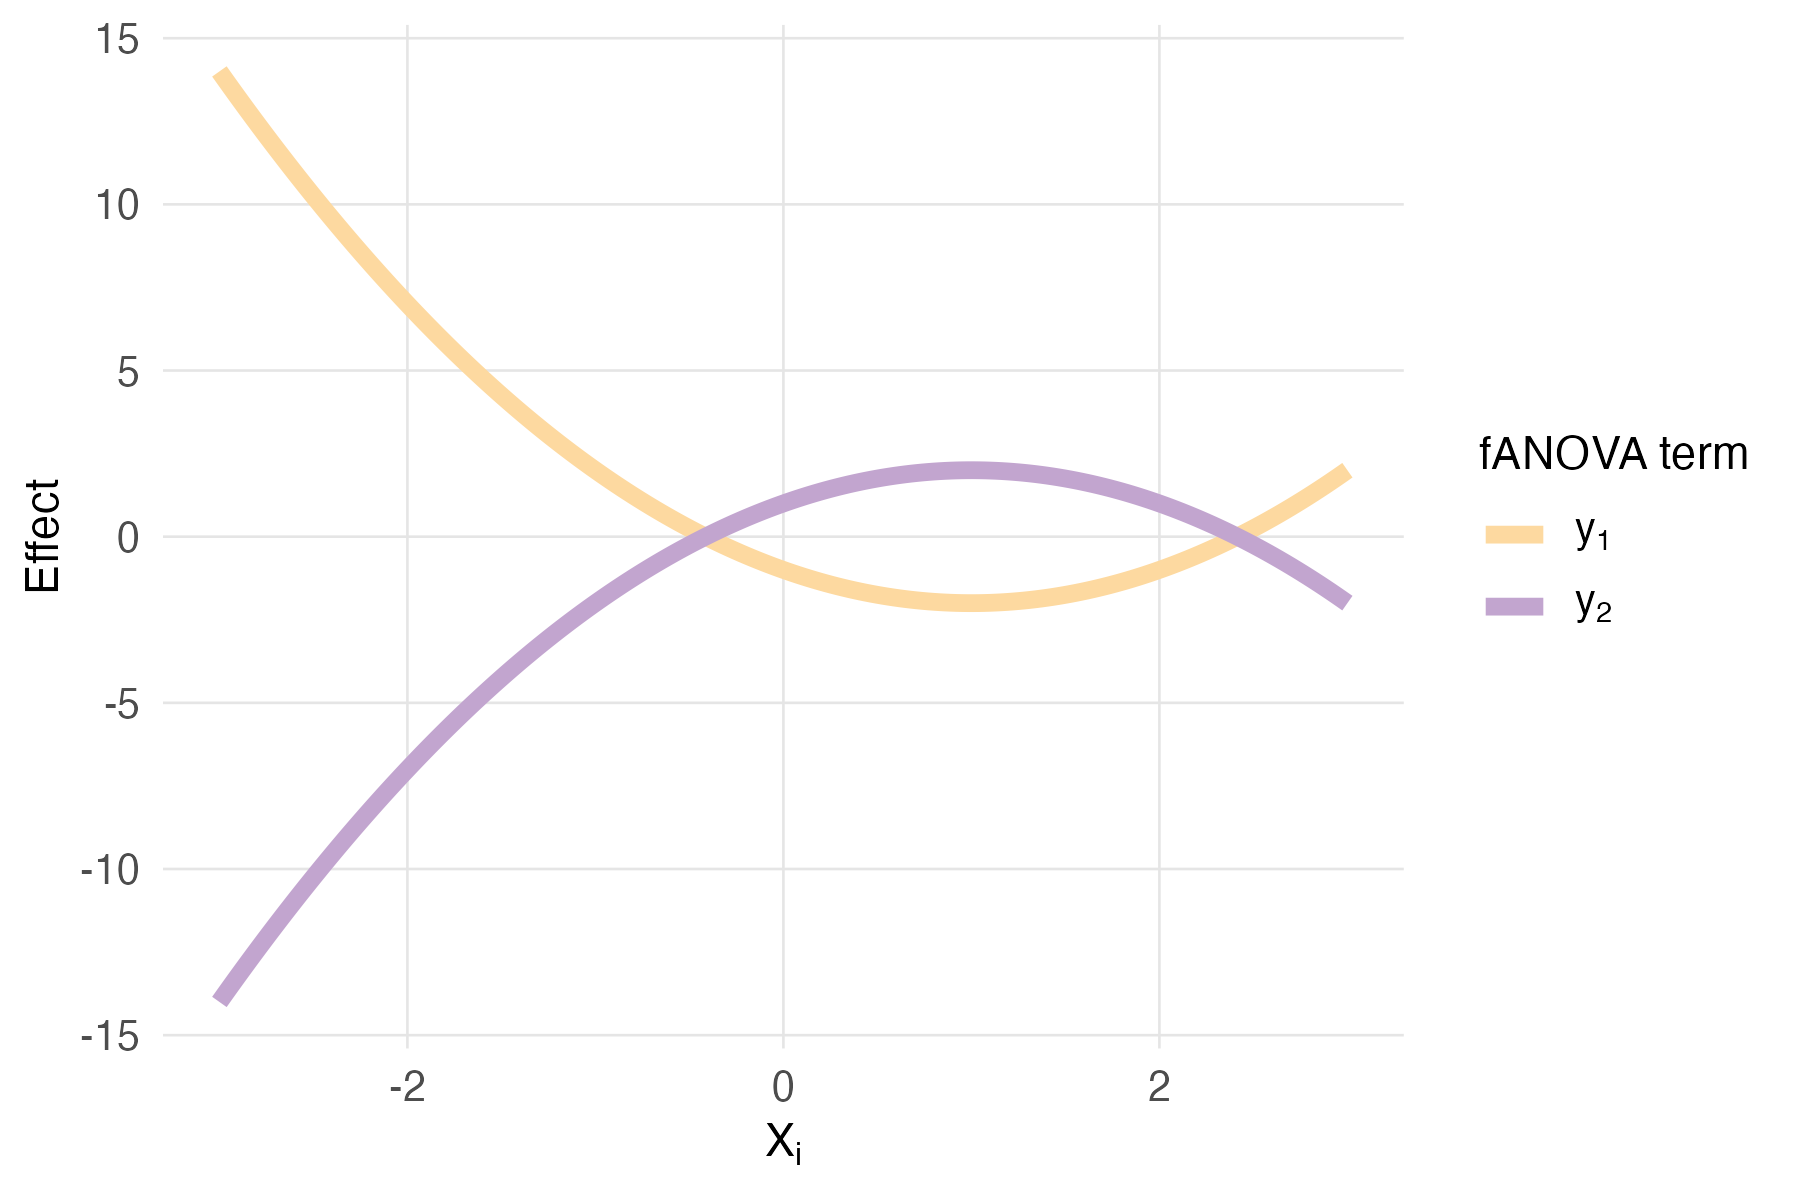
\includegraphics[width=\linewidth]{../images/experiment_section/mixed_a1m20_a2p20_a11p10_a22m10_a12p00_rhop00_main.png}
    \column{0.5\textwidth}
      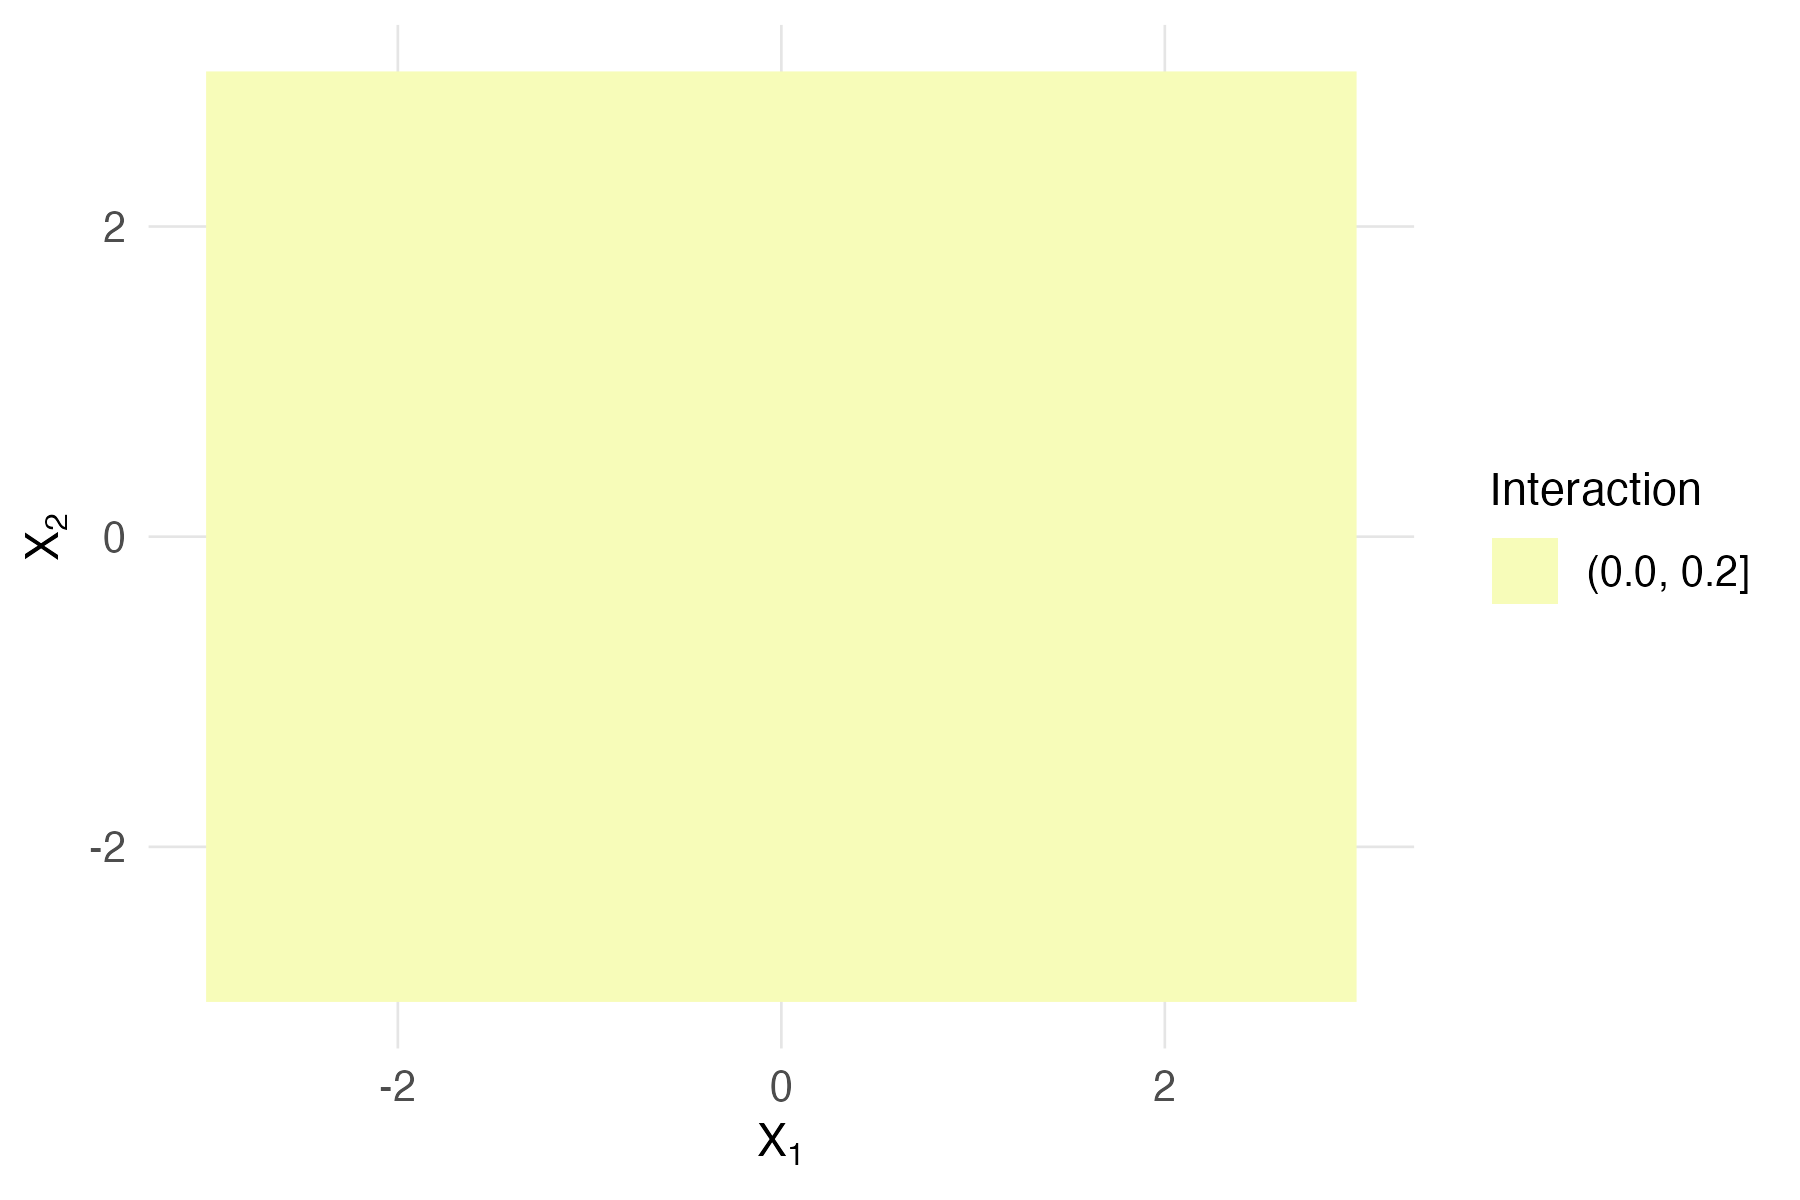
\includegraphics[width=\linewidth]{../images/experiment_section/mixed_a1m20_a2p20_a11p10_a22m10_a12p00_rhop00_interaction.png}
  \end{columns}
\end{frame}



\begin{frame}{Example: Only Linear Terms}
  \begin{columns}
    \column{0.5\textwidth}
      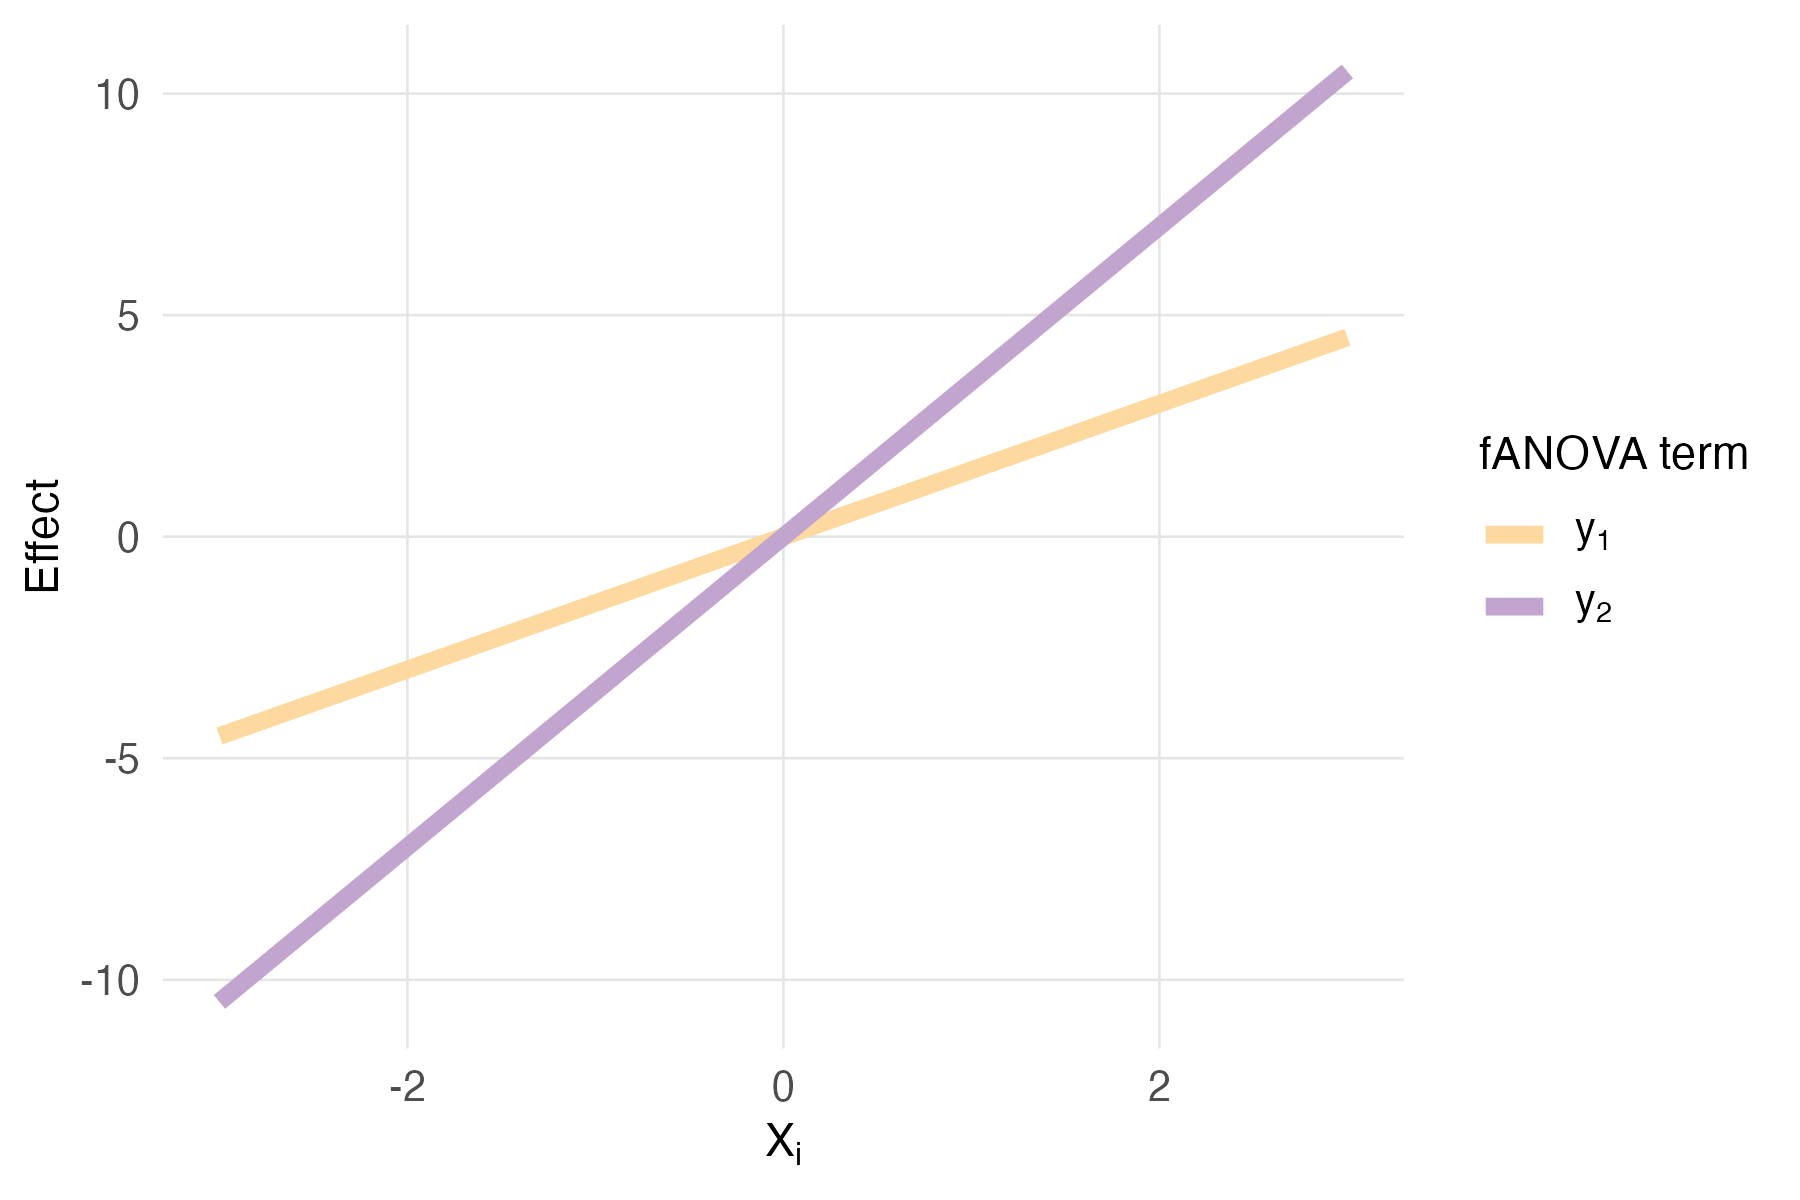
\includegraphics[width=\linewidth]{../images/experiment_section/linear_a1p15_a2p35_a11p00_a22p00_a12p00_rhop00_main.png}
      \captionof{figure}{$q(x_1, x_2) = 1.5 x_1 + 3.5 x_2$}
    \column{0.5\textwidth}
      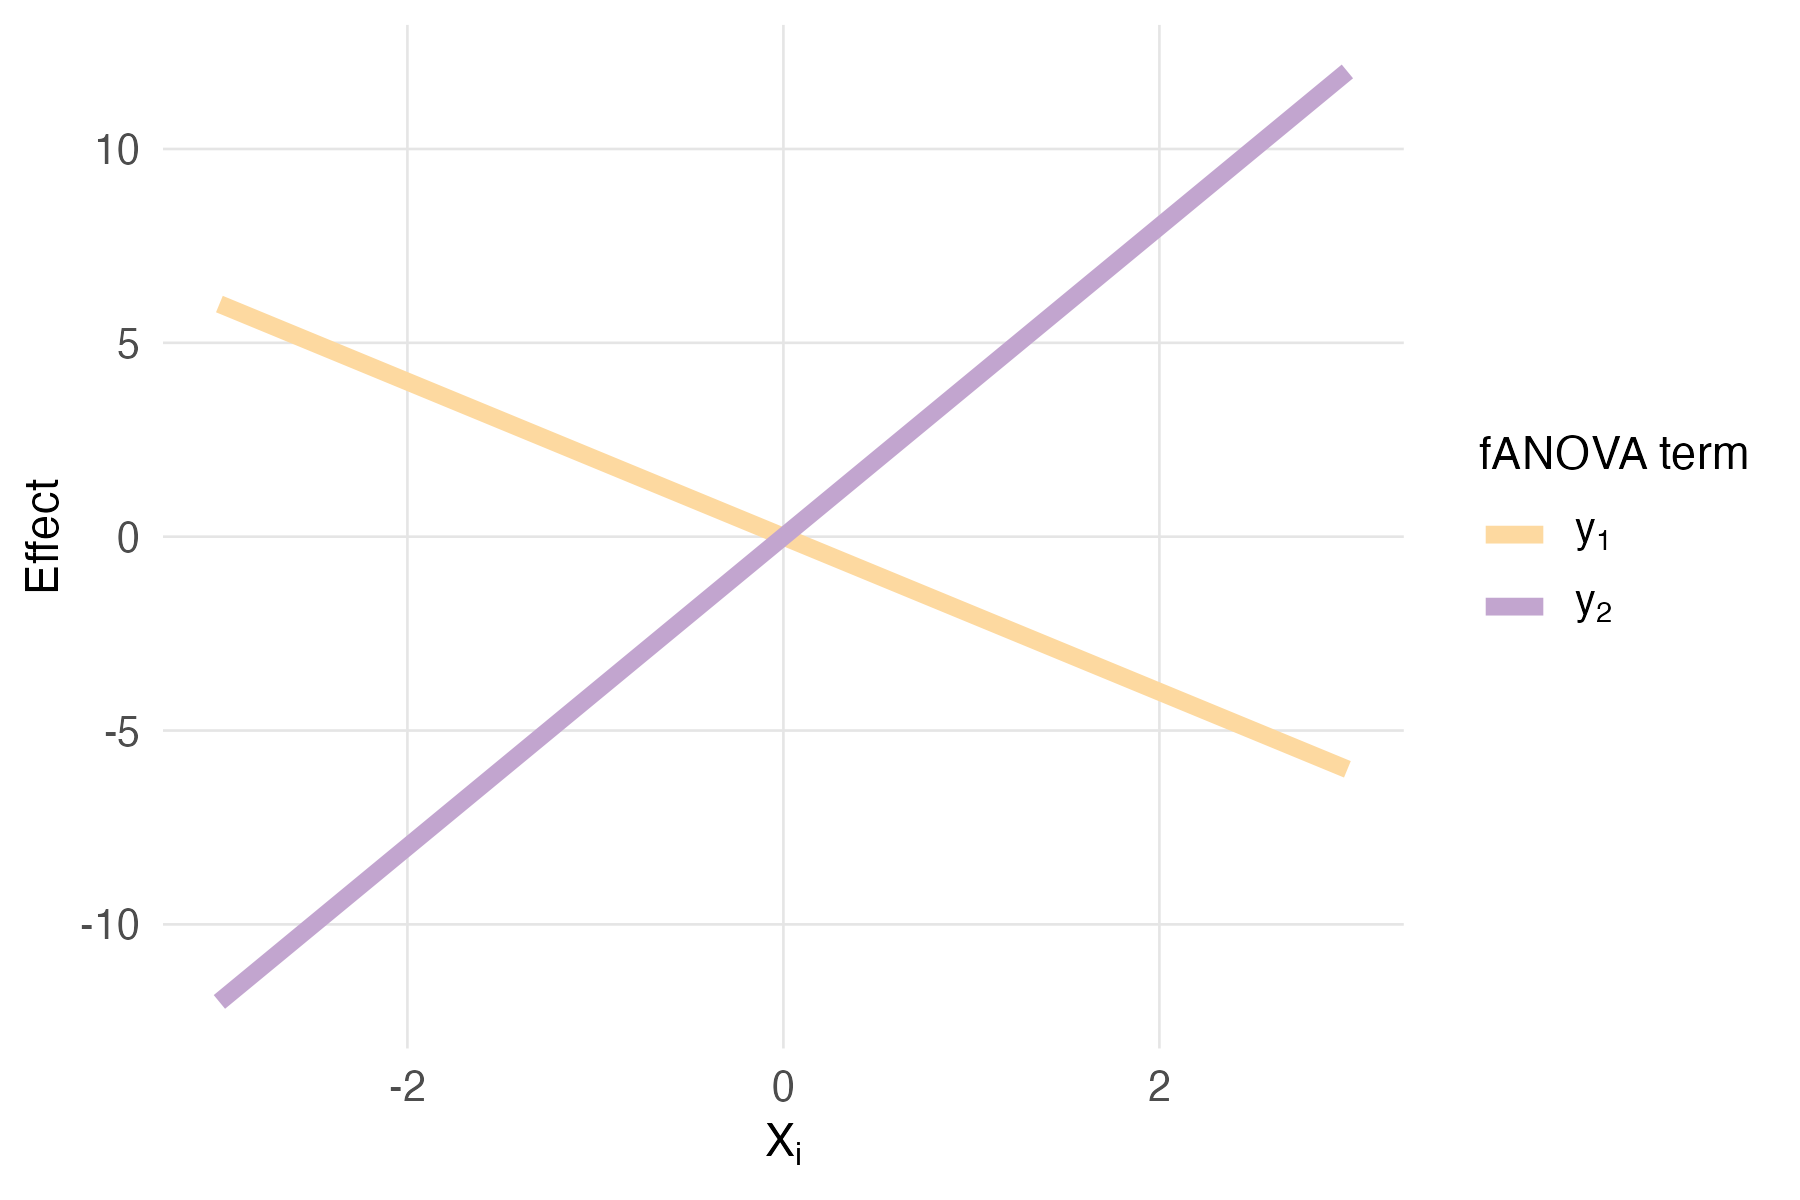
\includegraphics[width=\linewidth]{../images/experiment_section/linear_a1m20_a2p40_a11p00_a22p00_a12p00_rhop00_main.png}
      \captionof{figure}{$q(x_1, x_2) = -2 x_1 + 4 x_2$}
  \end{columns}
\end{frame}

\begin{frame}{Example: Interaction}
  \[
  y(x_1, x_2) = x_1 x_2 \qquad \rho = -0.5
  \]
    \begin{columns}
    \column{0.5\textwidth}
      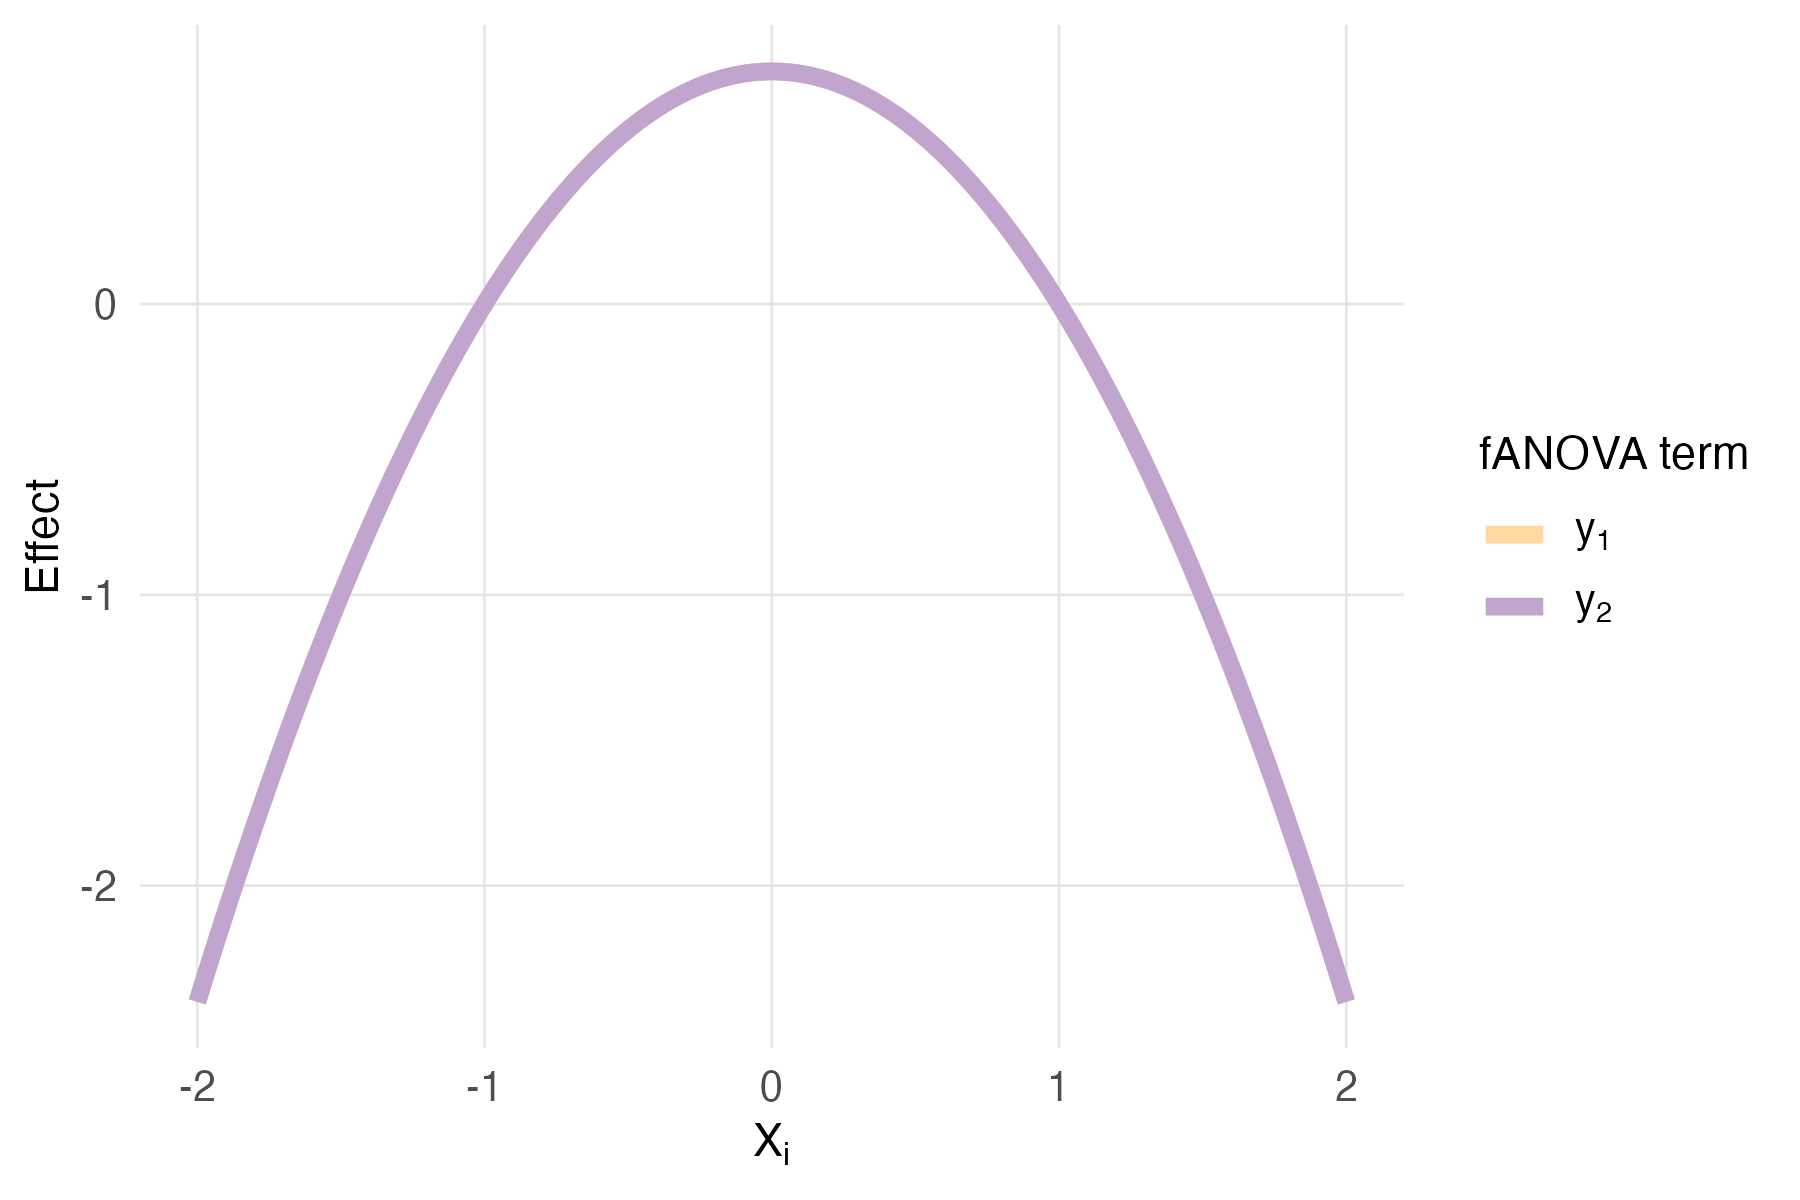
\includegraphics[width=\linewidth]{../images/experiment_section/interaction_a1p00_a2p00_a11p00_a22p00_a12p20_rhom05_main.png}
    \column{0.5\textwidth}
      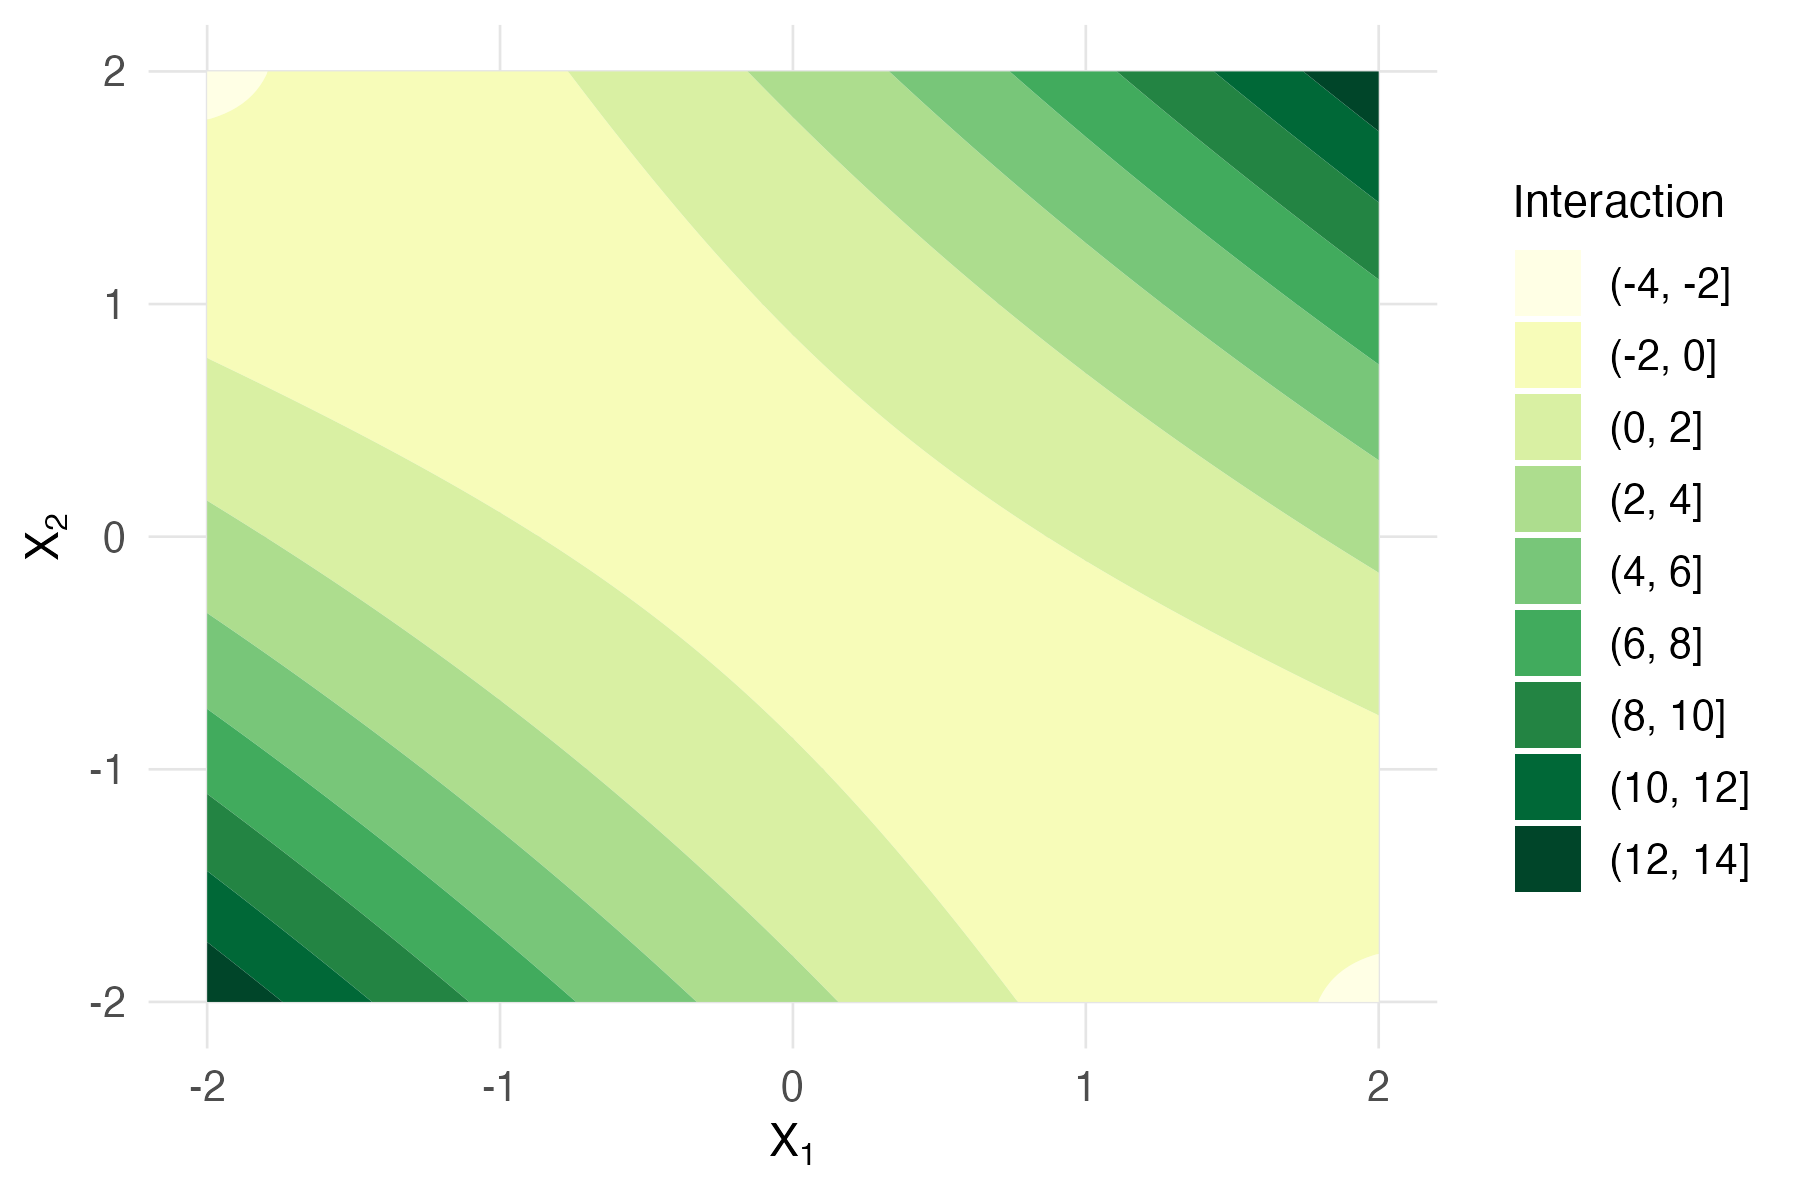
\includegraphics[width=\linewidth]{../images/experiment_section/interaction_a1p00_a2p00_a11p00_a22p00_a12p20_rhom05_interaction.png}
  \end{columns}
  
\end{frame}

\begin{frame}{Example: Interaction}
  \[
  y(x_1, x_2) = x_1 x_2 \qquad \rho = 0
  \]
    \begin{columns}
    \column{0.5\textwidth}
      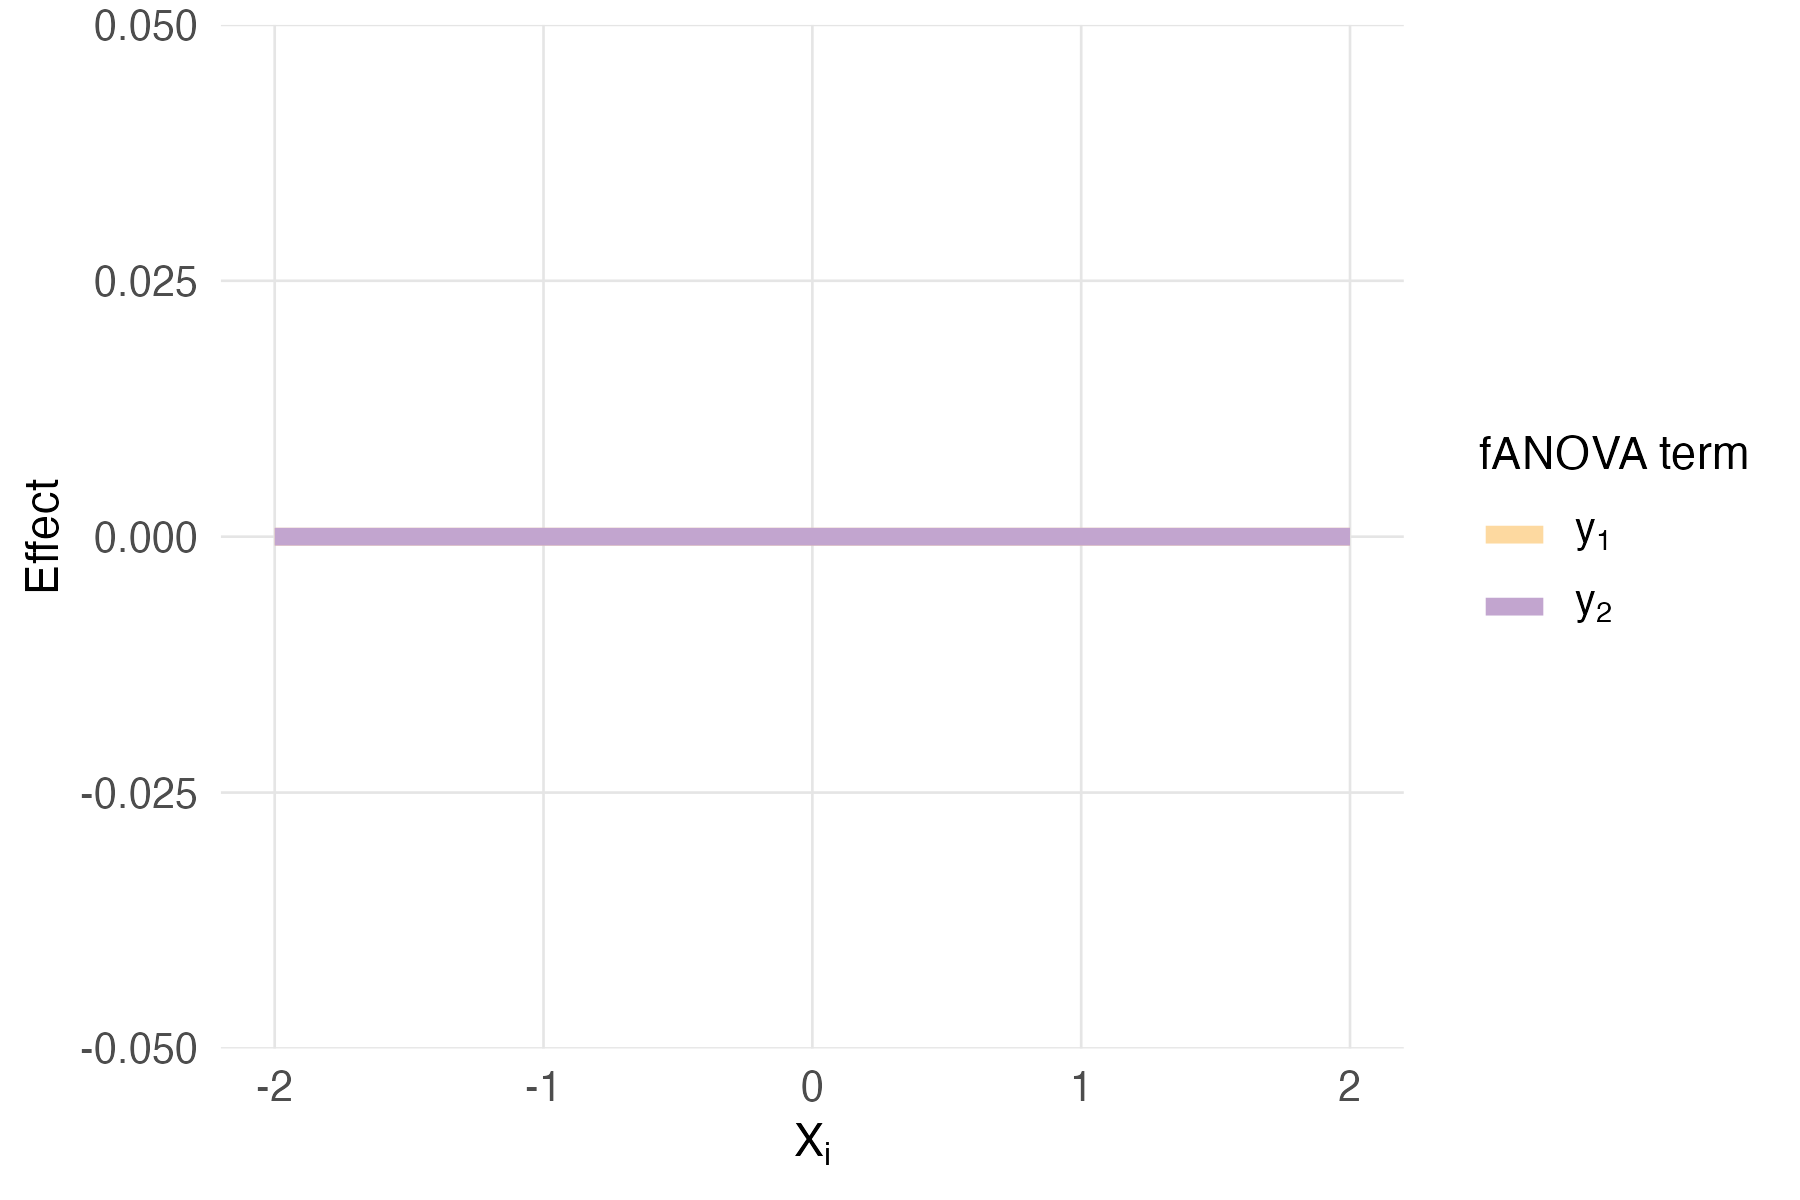
\includegraphics[width=\linewidth]{../images/experiment_section/interaction_a1p00_a2p00_a11p00_a22p00_a12p20_rhop00_main.png}
    \column{0.5\textwidth}
      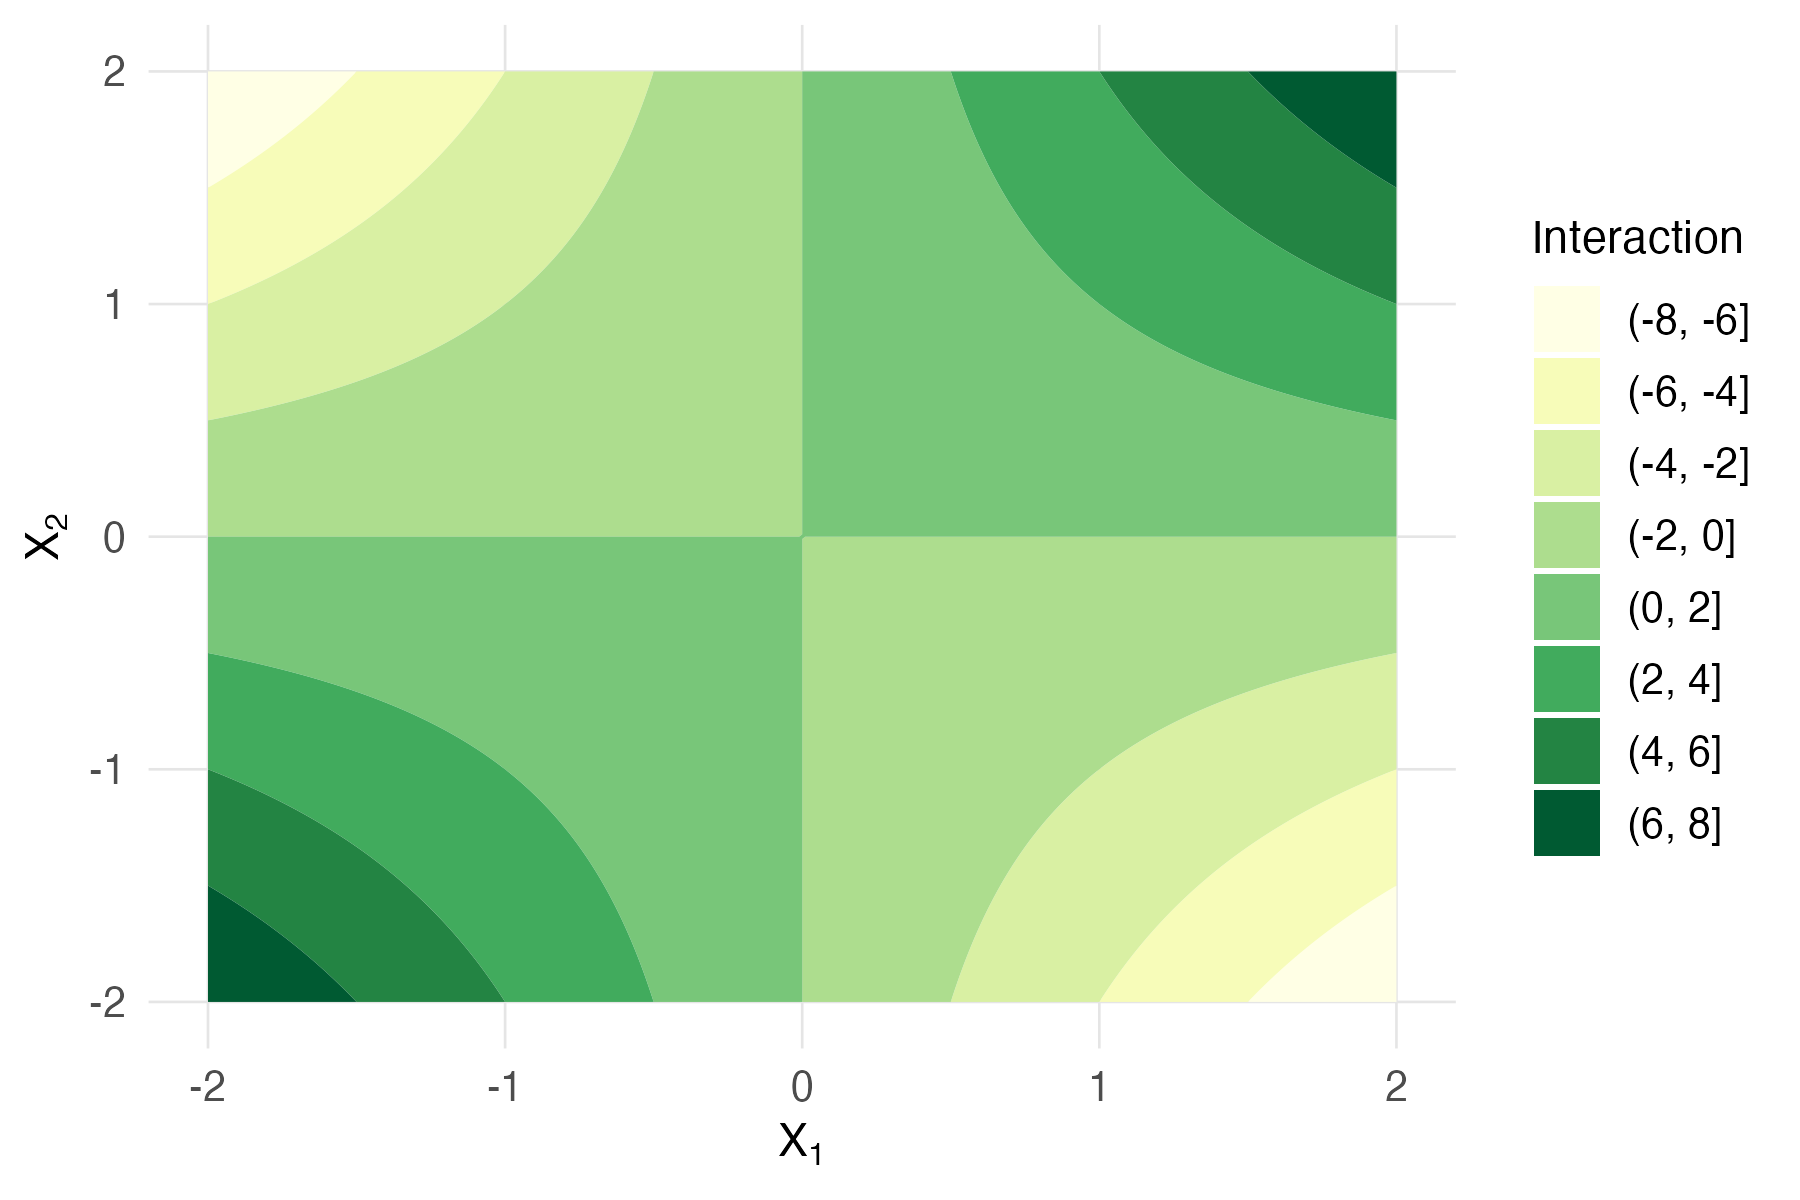
\includegraphics[width=\linewidth]{../images/experiment_section/interaction_a1p00_a2p00_a11p00_a22p00_a12p20_rhop00_interaction.png}
  \end{columns}
  
\end{frame}


\begin{frame}{Sobol Indices}
    Formula for classical Sobol' indices?
\end{frame}

\begin{frame}{Decomposition of linear functions}
  \begin{columns}
    \column{0.5\textwidth}
      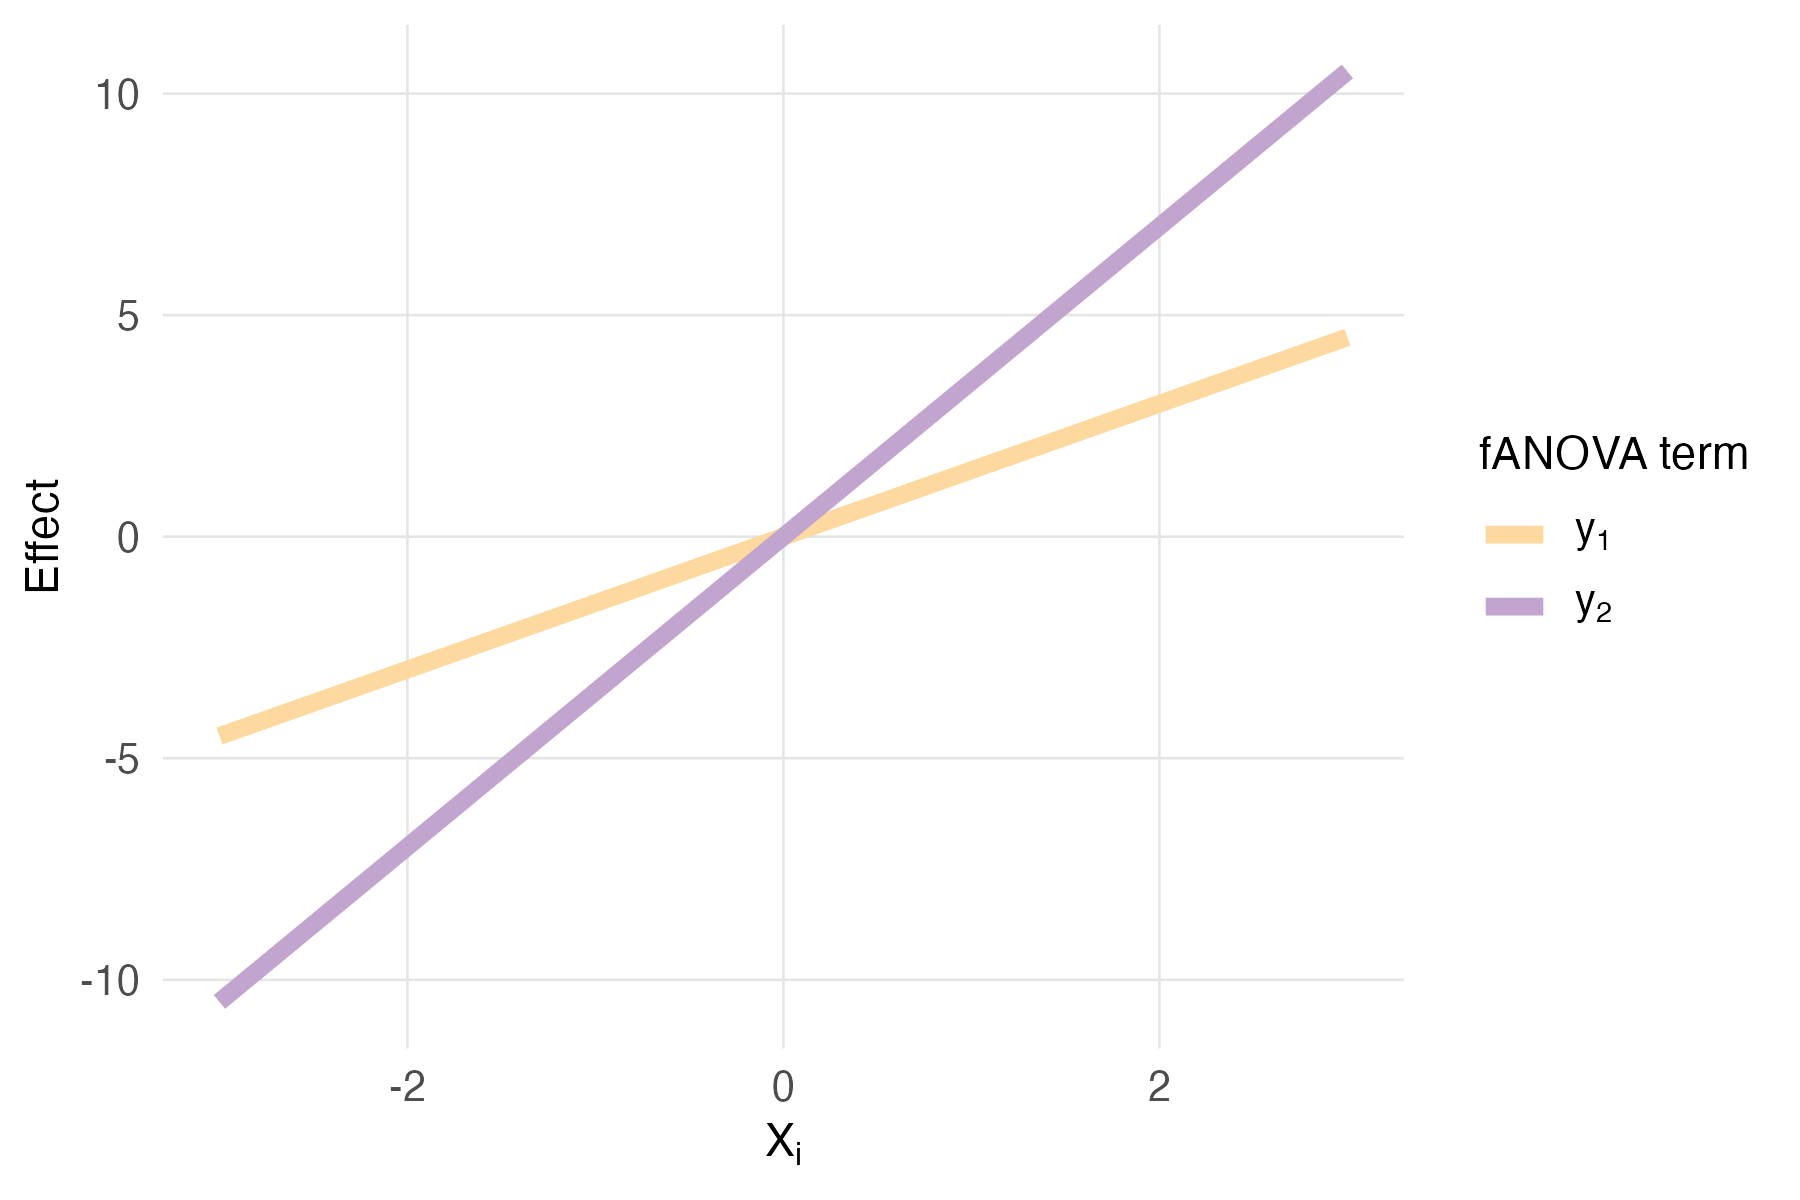
\includegraphics[width=\linewidth]{../images/experiment_section/linear_a1p15_a2p35_a11p00_a22p00_a12p00_rhop00_main.png}
      \captionof{figure}{$q(x_1, x_2) = 1.5 x_1 + 3.5 x_2$}
    \column{0.5\textwidth}
      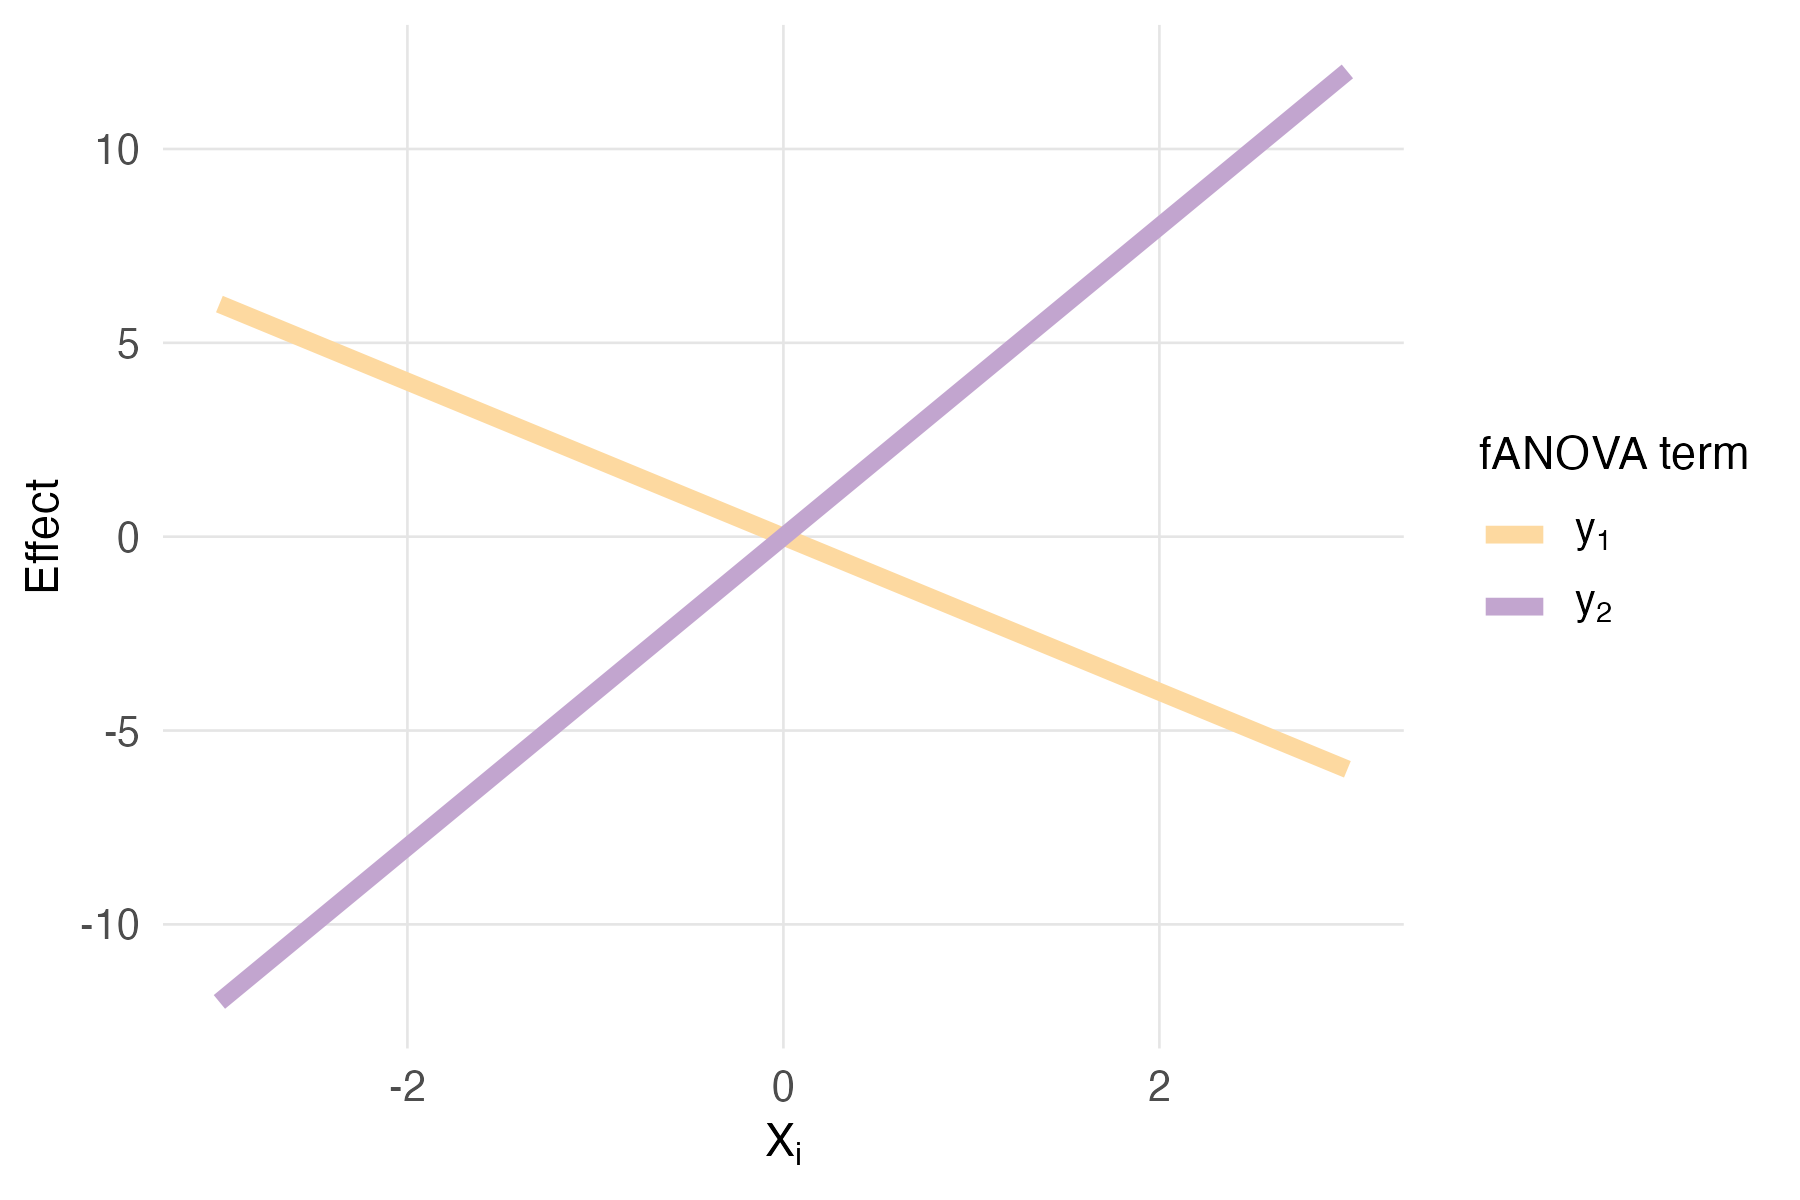
\includegraphics[width=\linewidth]{../images/experiment_section/linear_a1m20_a2p40_a11p00_a22p00_a12p00_rhop00_main.png}
      \captionof{figure}{$q(x_1, x_2) = -2 x_1 + 4 x_2$}
  \end{columns}
\end{frame}


\begin{frame}{Classical fANOVA Proofs}
    \begin{itemize}
        \item Zero mean property: factorized density, Fubinis Theorem, strong annihilating conditions
        \item Mutual orthogonality: factorized density, Fubinis Theorem, strong annihilating conditions
    \end{itemize}
\end{frame}

\begin{frame}{Generalized fANOVA Proofs}
    \begin{itemize}
        \item Zero mean property: separating $x$ into subvectors, marginal density, Fubinis Theorem, weak annihilating conditions
        \item Hierarchical orthogonality: set the scene, u is a proper subset of v $u \subsetneq v$, so there is an index in u which is not in v; divide $x_u$ into subvectors, marginal density, Fubini and weak annihilating conditions
        \item Weak annihilating becomes strong under independence: assume the weak ones, product density, factor out
        \item Three integration cases: distinguish between different relationships u and v, depending on the relationship the integral w.r.t. to marginal density simplifies
        \item Generalized fANOVA components by Rahman: first build constant term; for nonconstant terms use integration cases
        \item Integration constraint Hooker: show that hierarchical orthogonality is fulfilled if the conditions hold, show that it is not fulfilled if they do not hold; but why exactly these conditions a bit unclear
        \item Take a look at Sobols proof again
    \end{itemize}
\end{frame}

\begin{frame}{Relevant External Links}
    \begin{itemize}
        \item \url{https://docs.google.com/spreadsheets/d/1K5ECL6hDPDnHwM_k342xa29H-vHWzdk27PTgDHUwfFE/edit?usp=sharing} - Table with fANOVA-related literature
    \end{itemize}
\end{frame}